\chapter{Introduction}

\ifpdf
\graphicspath{{Chapter1/Figs/Raster/}{Chapter1/Figs/PDF/}{Chapter1/Figs/}}
\else
\graphicspath{{Chapter1/Figs/Vector/}{Chapter1/Figs/}}
\fi


Intelligent vehicles and transportation are attracting tremendous traction in recent years. These interests are not only limited to public perceptions and academia, but participations from major corporations beyond the automotive and computing industries are also greatly contributing toward the developments in this area. The solutions stemmed are actively deployed across various sectors, including transportation, mining, defence, agriculture, telecommunications, energy and trade. As a result, many new vehicles are progressively perceptive and autonomous; they are also becoming more environmentally friendly, often relying on renewable energy sources to mitigate their carbon footprint. It is therefore not uncommon to see them incorporating both elements into the same product. Case in point, many autonomous vehicles are electrically driven, such as the example given in Fig.~\ref{fig:1:bus}. It is often noticeable that autonomous, connected and electric vehicles are inextricably linked.

\begin{figure}[ht] 
	\centering    
	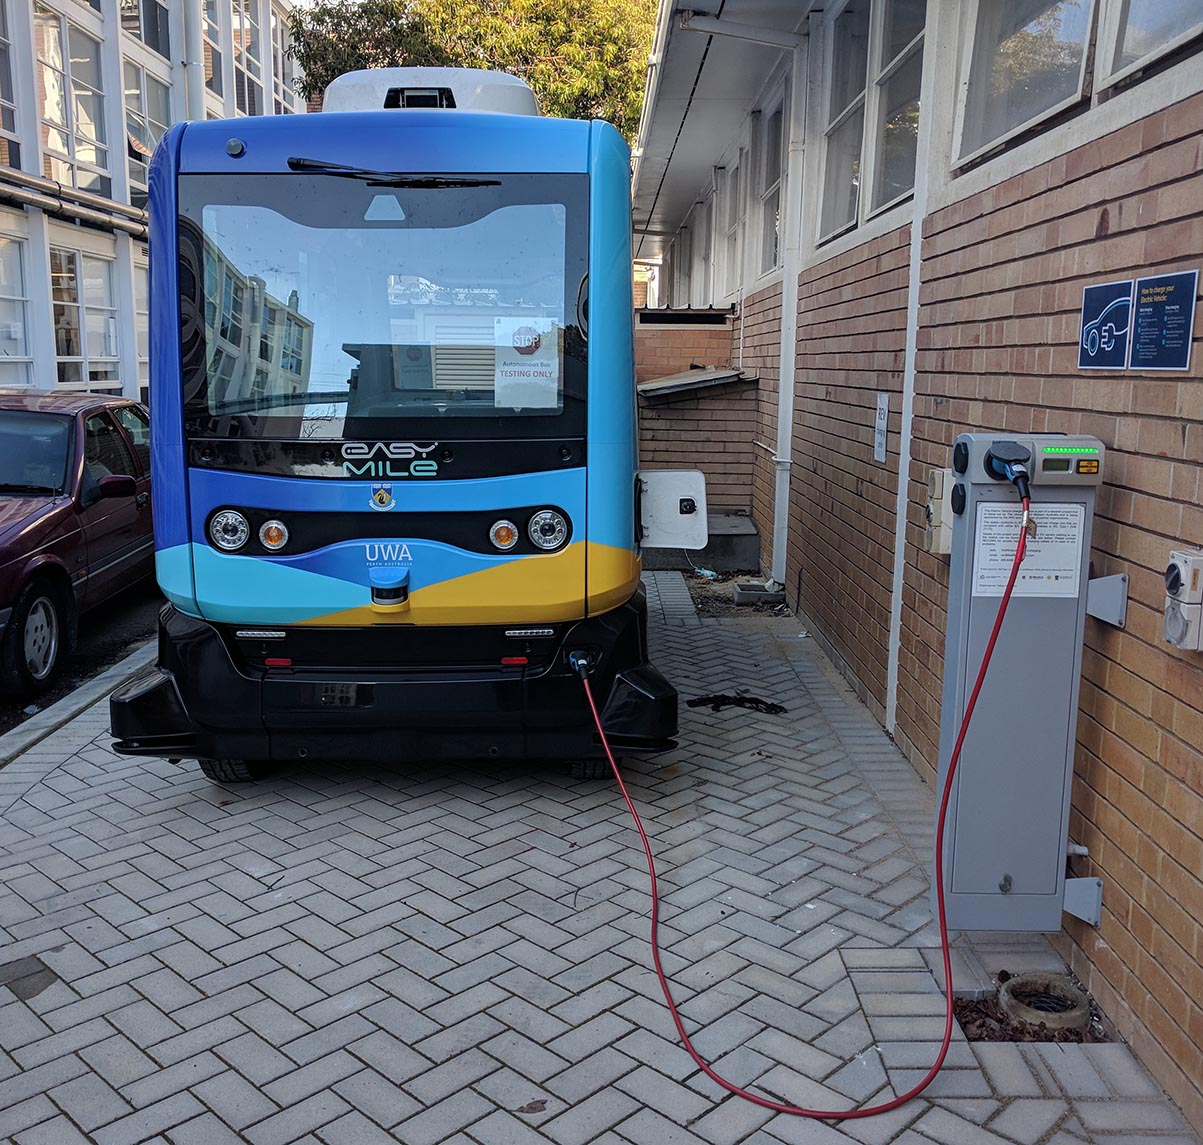
\includegraphics[width=0.6\textwidth]{bus}
	\caption{An EasyMile EZ10 driverless shuttle at a UWA charging station.}
	\label{fig:1:bus}
\end{figure}

\section{Autonomous Driving}
The general attainability of precise sensors and high performance compute hardware have driven recent interests in autonomous driving. Autonomous cars (also known as self-driving cars or driverless cars) perform autonomous driving by processing sensor data using an advanced control system that actively calculates the vehicle's navigation trajectory with obstacle avoidance. The sensors are often a combination of LiDARs, radars, sonar, GPS, local odometry, cameras and inertial measurement units (IMUs), which collectively compute through a process known as sensor fusion. Results from sensor fusion therefore enable the vehicle to achieve self-localisation or dead reckoning, along with scene understanding and object tracking. An example of an autonomous car is photographed in Fig.~\ref{fig:1:av}, showing its roof-mounted cameras and positioning sensors. 

\begin{figure}[ht] 
	\centering    
	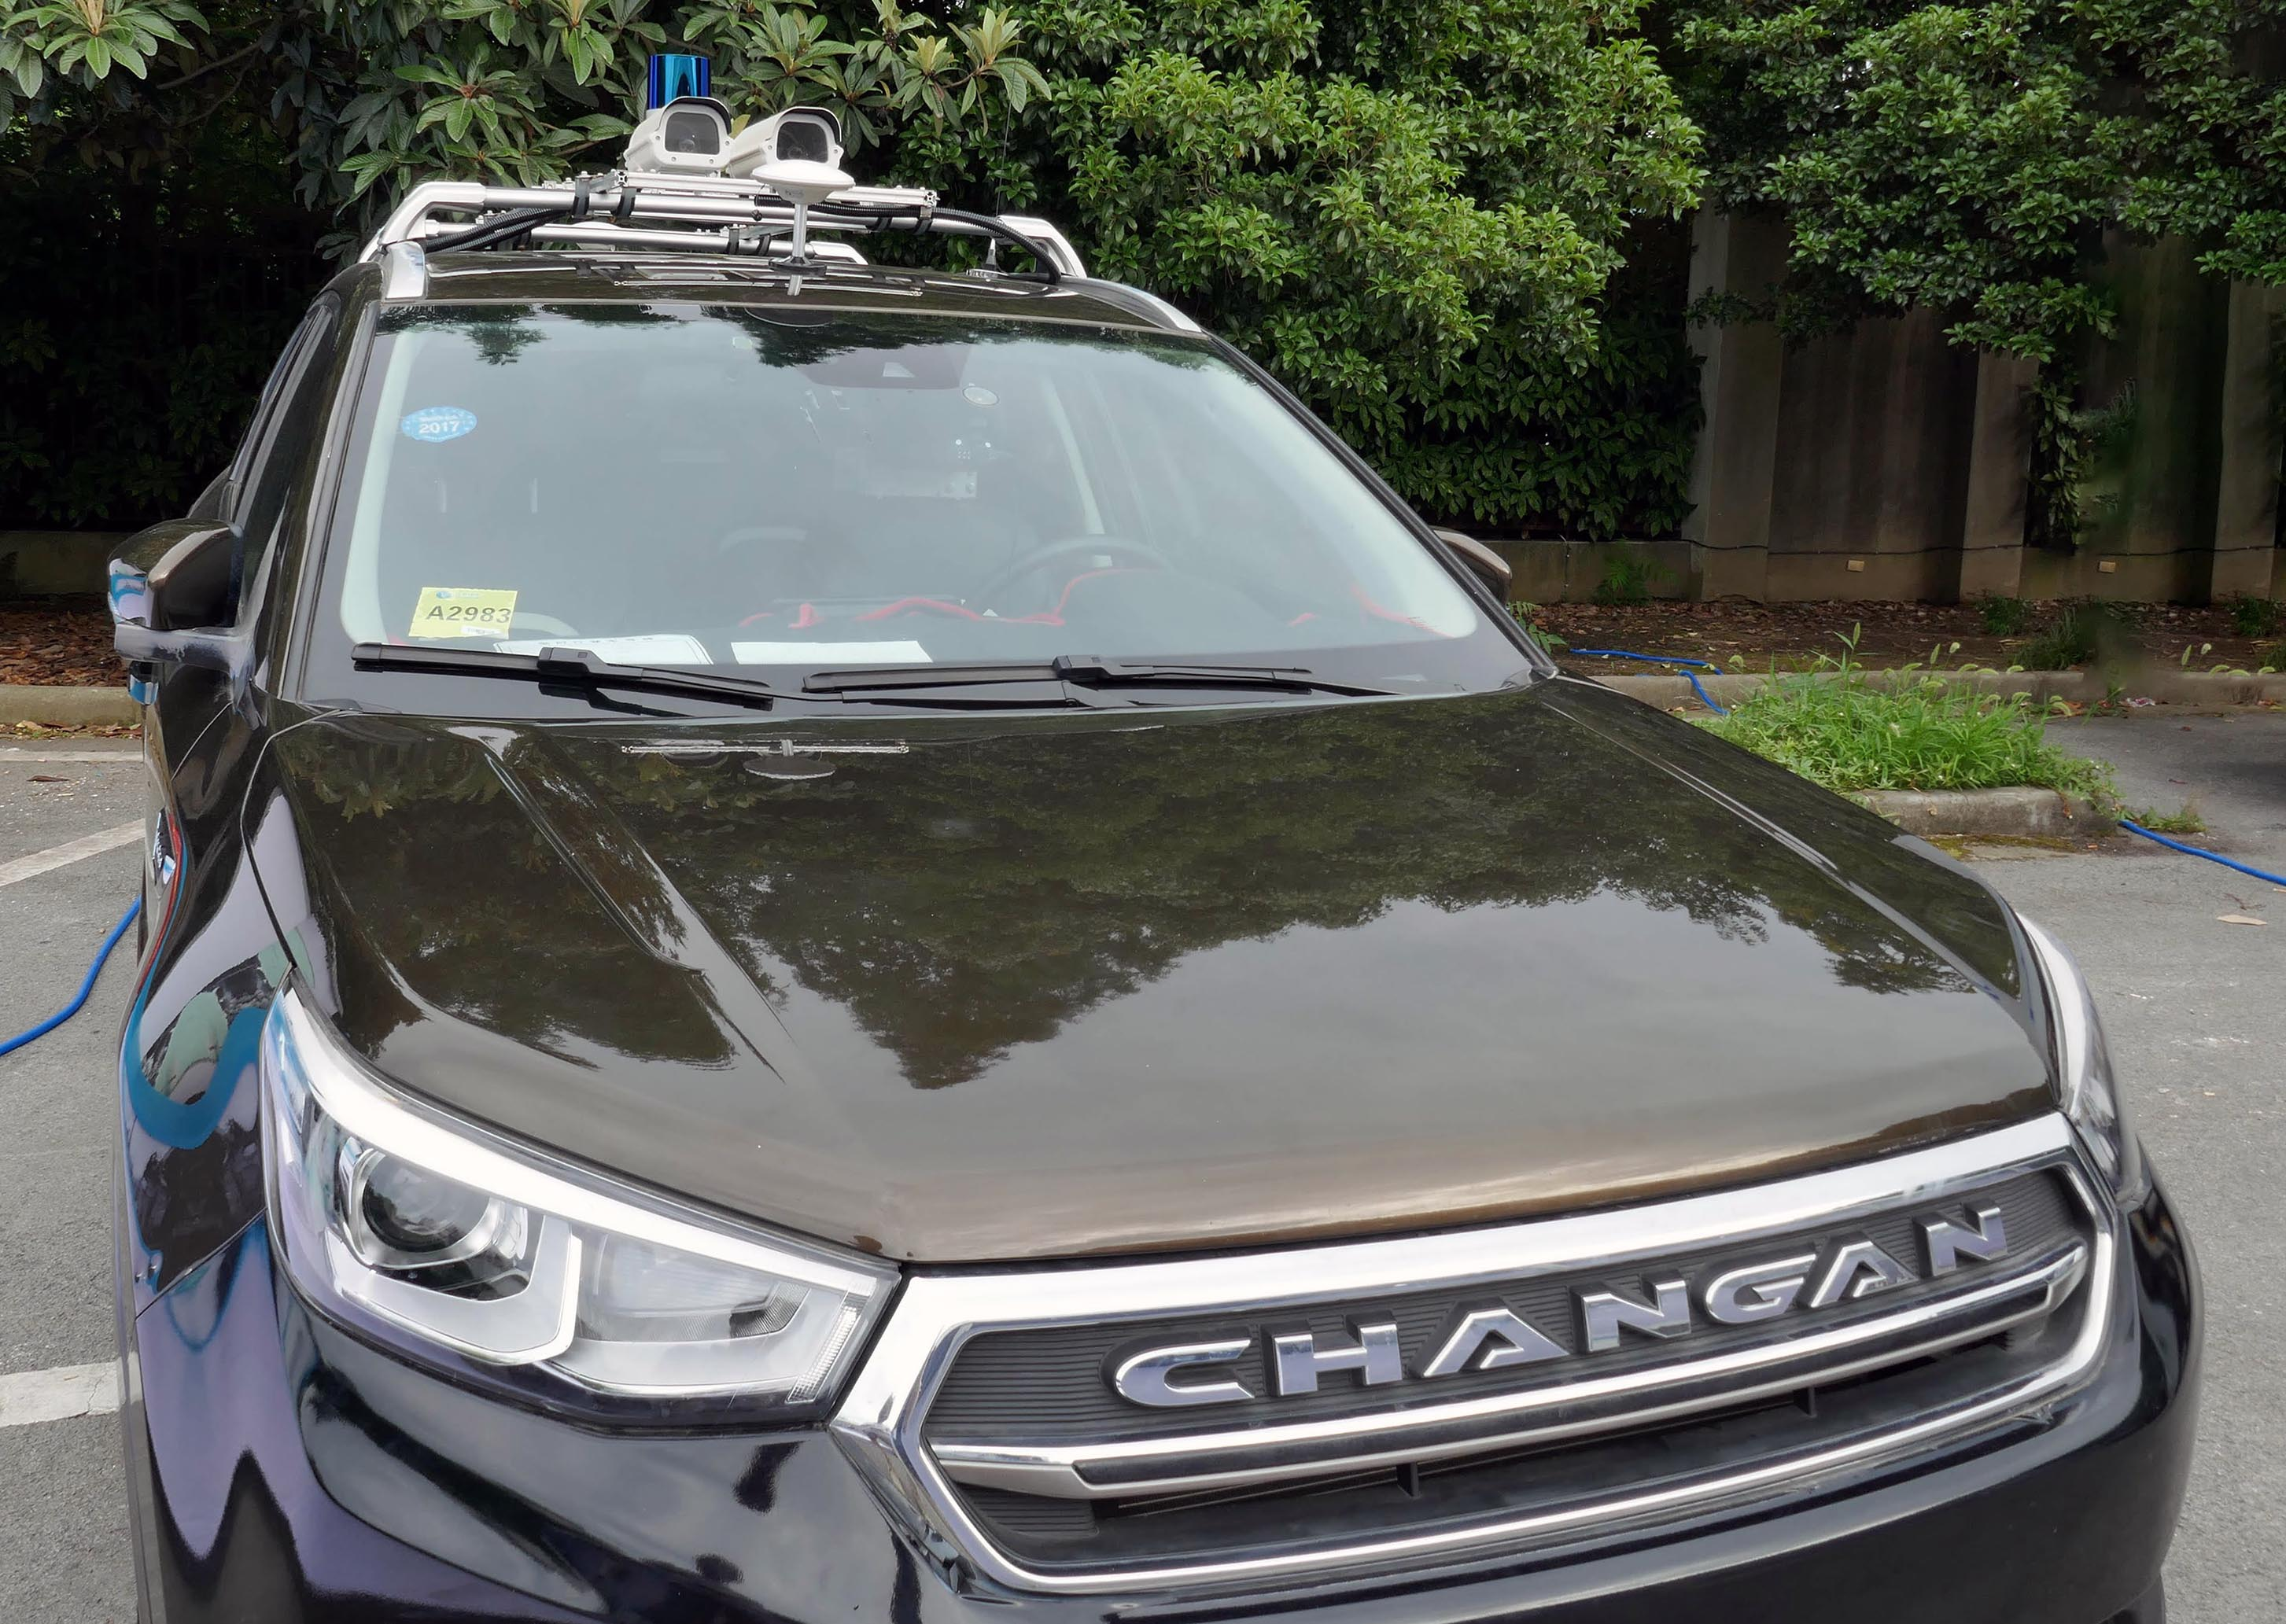
\includegraphics[width=0.7\textwidth]{av}
	\caption{An autonomous car with its sensors visibly mounted on its roof.}
	\label{fig:1:av}
\end{figure}

While autonomous cars have been developed as early as the 1980s~\cite{dickmanns_autonomous_1987}, many would argue that it was not until the DARPA Grand Challenge~\cite{buehler_2005_2007} before mainstream research into autonomous driving commenced. Since then, the developments in this area have been growing at a rapid pace. Market research reports published in 2018--2019~\cite{grand_view_research_self-driving_2018, kumar_autonomous_2018, htf_market_intelligence_overview_2019} have estimated the global capitalisation of autonomous vehicles to be valued at US\$55 billion in 2019, with a 35 per cent average compound annual growth rate (CAGR). Further, the Global Automotive \& Transportation Research Team at Frost \& Sullivan~\cite{frost_&_sullivan_global_2018} is expecting this figure to raise up to US\$173 billion by 2030, and also stated that shared mobility services such as ride-hailing are to contribute towards a 65 per cent share. 

Legislations pertaining to autonomous driving is also increasing in response to its growth. As of May 2019, according to the National Conference of State Legislatures (NCSL), 29 states in the United States have enacted autonomous vehicle legislations~\cite{hubbard_synthesis_2017}. The NCSL has also set up a publicly available Autonomous Vehicle State Bill Tracking Database that is easily searchable to cover various topics from commercialisation to vehicle testing~\cite{national_conference_of_state_legislatures_autonomous_2019}. In Australia, the National Transport Commission (NTC) has been tasked by the Australian Government to draft legislations relating to autonomous vehicles at the federal level~\cite{national_transport_commission_automated_2019}, including vehicle standards and safety concerns. This is performed while collaborating with various state governments, including Western Australia's Department of Transport~\cite{department_of_transport_automated_2018} to ensure nationwide consistency. %The REV Project at The University of Western Australia (UWA) actively participates 

%https://rosap.ntl.bts.gov/view/dot/35994s
%https://www.htfmarketreport.com/reports/1304659-global-self-driving-car-market-2
%https://www.mordorintelligence.com/industry-reports/autonomous-driverless-cars-market-potential-estimation
%https://www.grandviewresearch.com/industry-analysis/driverless-cars-market
%https://www.alliedmarketresearch.com/autonomous-vehicle-market

Safety is often a salient aspect of any successful development or legislation of autonomous vehicles. This landscape intends to minimise the human factor in driving, noting that human errors caused 94 per cent of all vehicle accidents in the United States~\cite{singh_critical_2015}, which would imply that an ideal autonomous vehicle penetration will reduce accidents by up to 90 per cent~\cite{bertoncello_ten_2015}. Similarly, 51 per cent of road fatalities in Australia are caused by the driver in 2018~\cite{department_of_infrastructure_transport_cities_and_regional_development_safety_2019}. In order to encourage the penetration and public perception towards autonomous vehicles, MIT's Technology Review has noted the lack of an industry standard for the safety of autonomous vehicles, and have published a brief report relating to the safety regulations~\cite{mit_technology_review_insights_autonomous_2019}. 

%https://crashstats.nhtsa.dot.gov/Api/Public/ViewPublication/812115
%https://www.bitre.gov.au/statistics/safety/

With the economics, legislation and safety setting the development baseline, autonomous driving applications have since evolved from advanced driver-assistance systems (ADAS), where it initially incorporated features including adaptive cruise control, automated parking, blind spot detection, lane departure warning, automatic lane centring and collision avoidance. Driving automation often consolidates these features with active navigation and control, minimising the need for driver intervention. To this end, SAE International has classified driving automation into five different levels under its J3016 ``Levels of Driving Automation'' standard, ranging from Level 0 (manual driving) to Level 5 (fully autonomous driving)~\cite{on-road_automated_driving_orad_committee_taxonomy_2018}. %SAE Report downloaded
The official SAE J2016 graphic is given as Fig.~\ref{fig:1:j3016}. An increase in driving automation level would typically require greater computation complexity, often using more sensors than its preceding level. Automotive manufacturers have begun the inclusion of Level 3 automation features in production vehicles since 2018, most notably with Tesla's Autopilot feature. 

\begin{figure}[H] 
	\centering    
	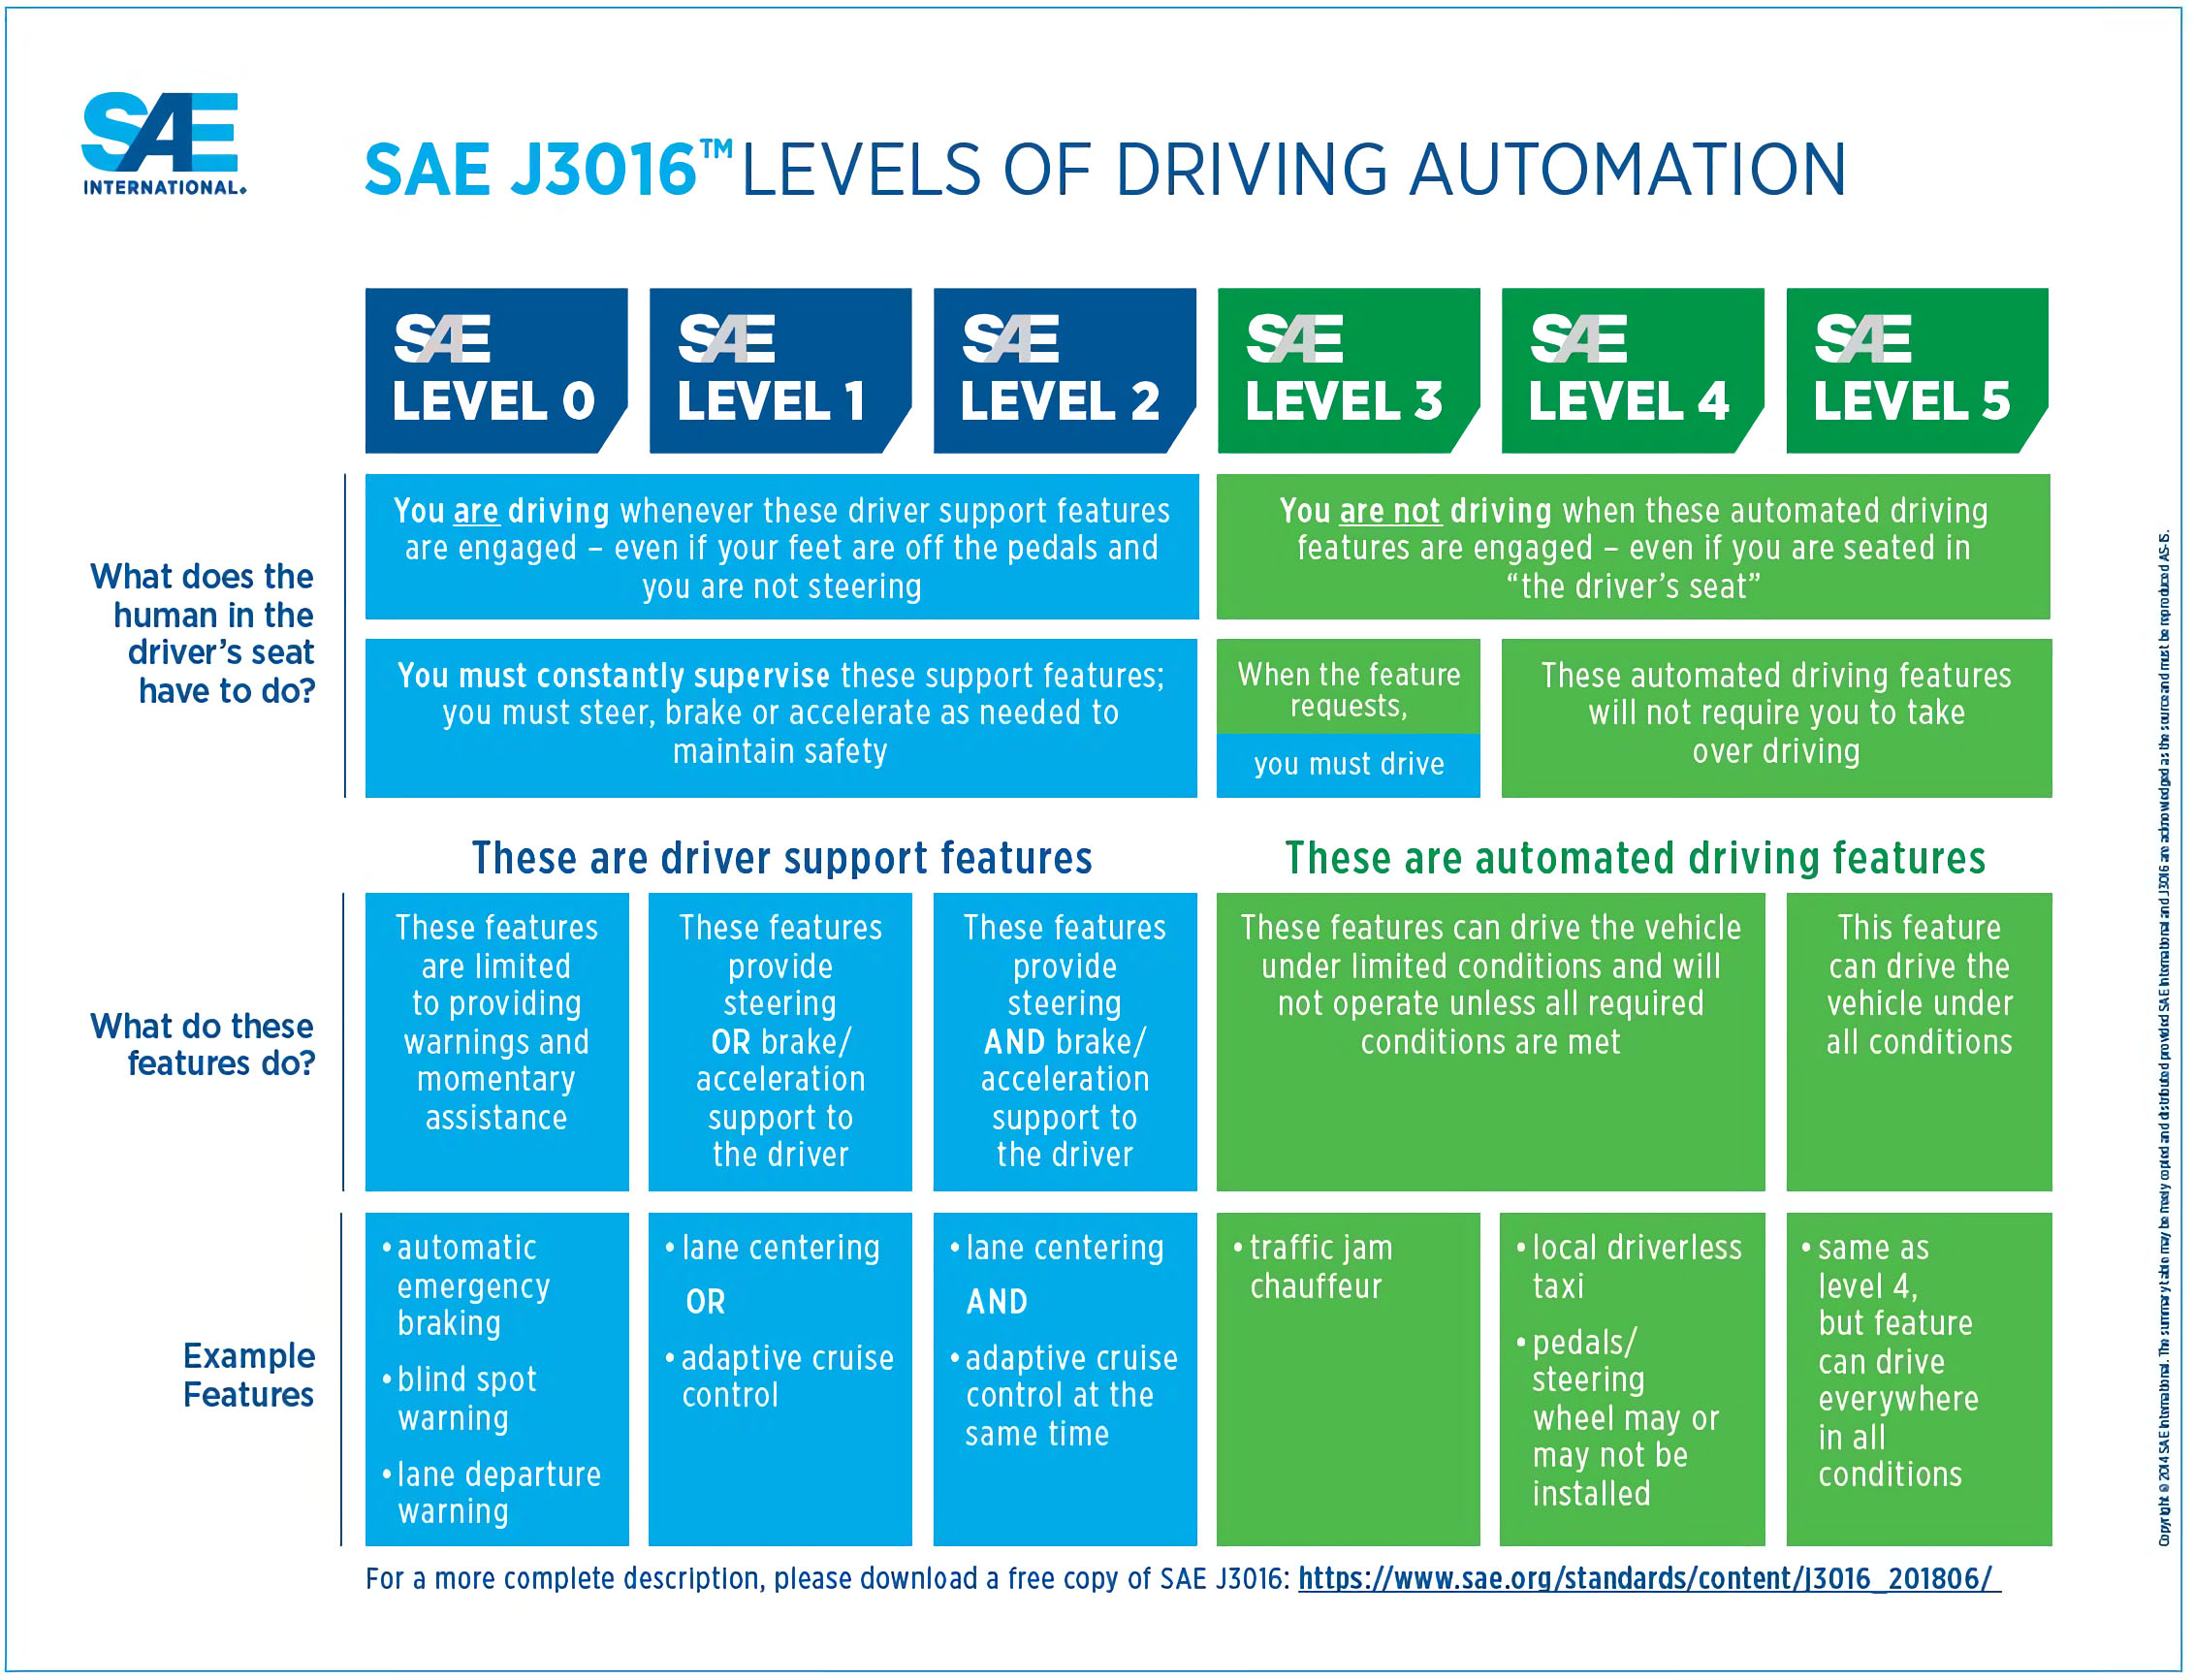
\includegraphics[width=\textwidth]{j3016}
	\caption[SAE J3016 official graphic]{The official graphic for the SAE J3016 standard as of January 2019~\cite{shuttleworth_sae_2019}.}
	\label{fig:1:j3016}
\end{figure}

Trials for Level 4 and 5 automation are being conducted by technological corporates such as Google (Waymo) and Uber. It is currently less favoured by production vehicles as the addition of high accuracy sensors would render the ownership cost prohibitive. In the case of positioning, conventional GPS devices have a reporting accuracy of approximately 10 metres, which is inadequate for autonomous navigation; many applications instead use differential GPS or real-time kinematic (RTK) to obtain accurate positioning, incurring higher implementation costs. On the perception front, vehicles often use LiDARs or radars to survey their immediate environment, thereby enabling them to detect or classify objects, and perform obstacle avoidance when necessary. LiDARs are typically preferred over radars in for object tracking and mapping, as it provides distance measurements accuracies in the order of millimetres. They are also capable of producing high definition maps, enabling precise localisation for the vehicles. These vehicles often install multiple LiDARs on their chassis to achieve a \ang{360} perception of its surroundings, often in addition to having dedicated LiDARs for mapping. This further increases the implementation costs, especially considering that individual LiDARs often cost tens of thousands of dollars. 

Due to the lower cost of cameras compared to LiDARs, newer applications are starting to favour using the camera as the vehicle's main perceptive sensor. These applications use computer vision methods to achieve localisation and object classification, often through a single input. However, computer vision algorithms are often more complex, requiring greater computation and memory footprints. This is particularly true when compared against LiDAR-based methods, as they only output a series of measurements, as opposed to a series of complete images that a camera outputs. Nevertheless, with the arrival of high-performance parallel computers, computer vision methods are more likely to better utilise these hardware platforms to achieve more desirable outcomes. These methods have been demonstrated to deliver results pertaining to accurate localisation, mapping and scene understanding; ideally replacing the need for LiDARs, radars, IMUs and local odometry. Using the cameras offer a more cognitive approach to autonomous driving, whereby it mimics a human's visual perception of the world while driving. Tesla has always maintained a critical position towards LiDARs and favouring the cameras due to its cost and due impracticality, with its CEO Elon Musk claiming that ``Anyone relying on LiDAR is doomed'', during his keynote address at the 2019 Tesla Autonomy Investor Day~\cite{burns_anyone_2019}.

This thesis describes works that contribute towards using the camera as the primary sensor for autonomous driving, viz. visual autonomous driving. By evaluating these algorithms on the testbed shown in Fig.~\ref{fig:1:sae}, it was found that algorithms relating to environmental perception and localisation can be substituted with computer vision methods. For instance, visual odometry is used in place of wheel odometry and inertial measurements; object classification, detection and tracking be done using the camera in place of LiDARs. Computer vision methods are therefore more versatile as multiple algorithms are able to leverage on a single data source. By doing so, these sensors can then supplement computer vision measurements as an alternative to improve upon classification or measurement accuracies. 

\begin{figure}[ht] 
	\centering    
	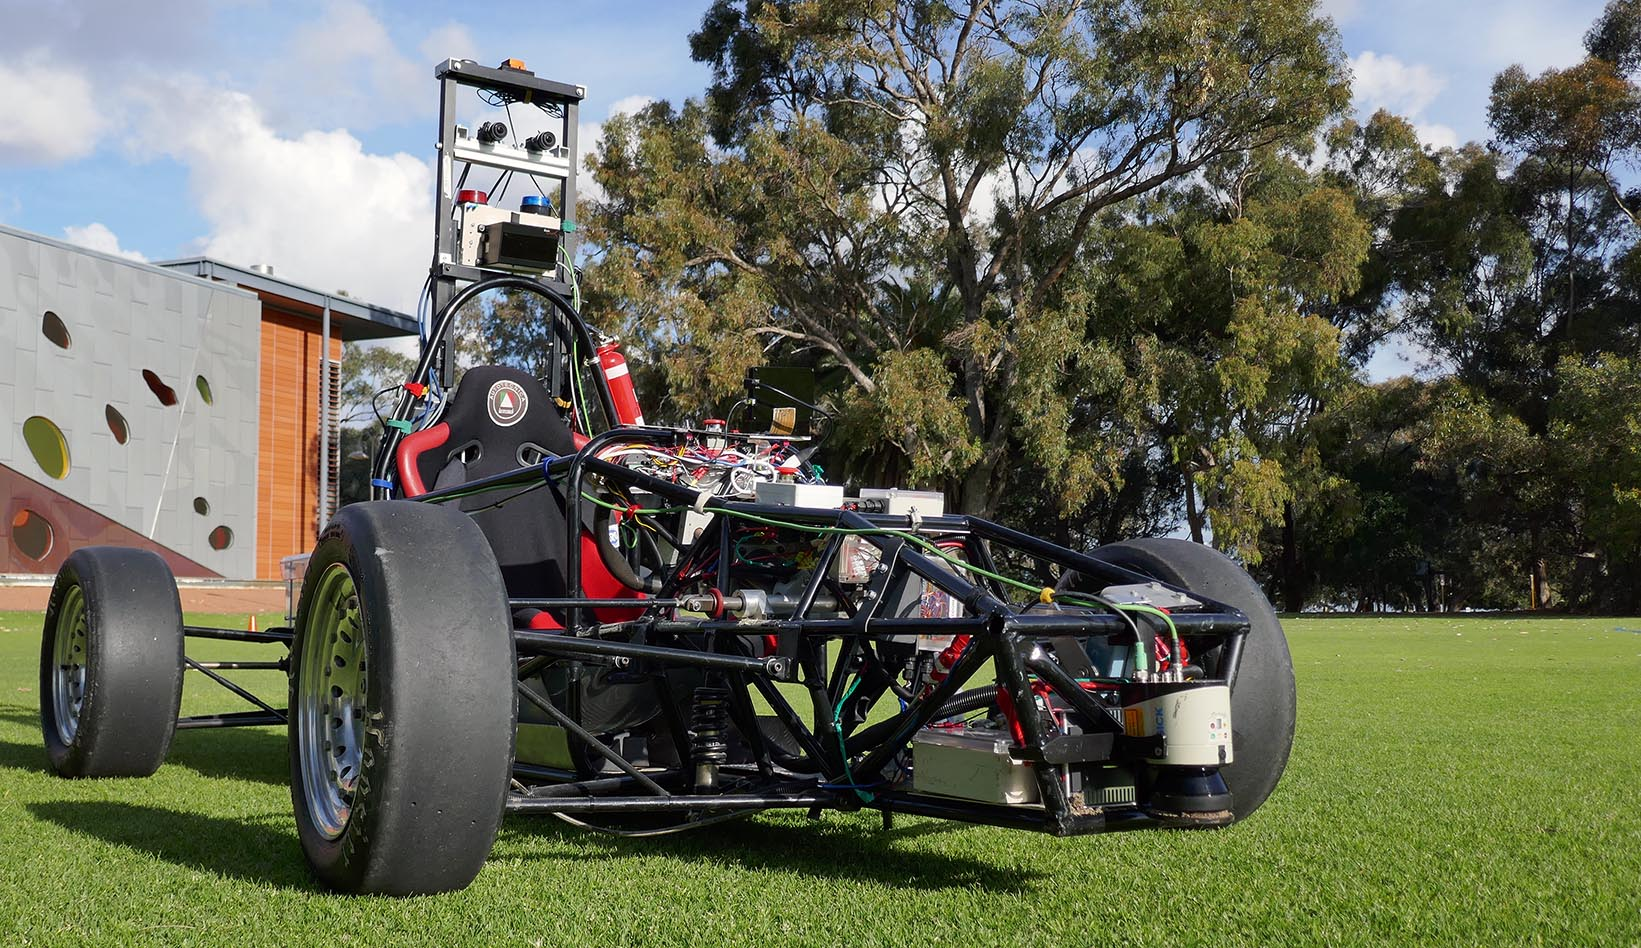
\includegraphics[width=0.7\textwidth]{sae}
	\caption{The REV Project's autonomous Formula SAE Electric test vehicle.}
	\label{fig:1:sae}
\end{figure}

\nomenclature[z-lidar]{LiDAR}{Light Detection and Ranging} 
\nomenclature[z-gps]{GPS}{Global Positioning System} 
\nomenclature[z-imu]{IMU}{Inertial measurement unit} 
\nomenclature[z-cagr]{CAGR}{Compound annual growth rate} 
\nomenclature[z-ncsl]{NCSL}{National Conference of State Legislatures} 
\nomenclature[z-darpa]{DARPA}{Defense Advance Research Projects Agency} 
\nomenclature[z-adas]{ADAS}{Advanced driver-assistance systems} 
\nomenclature[z-rtk]{RTK}{Real-time kinematic (positioning)} 


%history, OEMs, safety, levels SAE, future applications
\section{Electromobility}
The increased awareness of climate change at the turn of the century is contributing to the rise in sustainable and renewable energy sources worldwide. Heightened levels of greenhouse gas emissions have prompted international treaties, most notably the United Nations Framework Convention on Climate Change (UNFCCC). The UNFCCC Paris Agreement saw 195 ratifications to tackle issues relating to global warming, with a focus to reduce greenhouse gas emissions, and to increase the share of renewable energy and energy efficiency, limiting warming to under 1.5--2°C~\cite{rogelj_paris_2016}. This agreement came into force on 4 November 2016. Carbon dioxide (CO\textsubscript{2}) remains by far the largest contributor to greenhouse gas emissions (82 per cent)~\cite{united_states_environmental_protection_agency_inventory_2019}. In part, transport is responsible for 23 per cent of global emissions, and is projected to increase to 50 per cent by 2050; car emissions constitute half of this figure~\cite{santos_road_2017}. In Australia, transport remains the second largest source of greenhouse gas in the country, emitting 102 million tonnes (18 per cent) of CO\textsubscript{2} in 2018, and is projected to reach 111 million tonnes by 2030 at its current rate~\cite{department_of_the_environment_and_energy_australias_2018}. 

%https://unfccc.int/resource/docs/2015/cop21/eng/l09r01.pdf
%https://www.epa.gov/ghgemissions/inventory-us-greenhouse-gas-emissions-and-sinks
%https://www.sciencedirect.com/science/article/pii/S0967070X17304262
%https://www.environment.gov.au/system/files/resources/128ae060-ac07-4874-857e-dced2ca22347/files/australias-emissions-projections-2018.pdf

Noting that a vehicle's CO\textsubscript{2} emissions increases with its fuel consumption and type, the automotive industry is making efforts to reduce the carbon footprint of production vehicles with the introduction of green vehicles that run on alternative fuels, including electricity. Electromobility (or e-mobility) is a portmanteau of electric and mobility that is often used to describe electric driving in light of its renaissance that began in the late 2000s. Since the late 2010s, it is mainly used to describe electric vehicles (EVs), particularly electric cars as a relation to current motoring trends.

Electromobility was first conceptualised in the 1900s, back when climate change was unlikely to be a concern. The rationale to produce electric cars back then was to mitigate rising fossil fuel prices while being less noisy. However, it was quickly phased out of favour due to subsequent advancements with the internal combustion engine (ICE)~\cite{kirsch_electric_2000}. Still, the availability and know-hows in electromobility continued to persist and improve over the years with overhead line-based transportation, and components such as motors and controllers have become faster and more efficient. Throughout the century, several attempts have been made to reintroduce electric driving to the market, more recently with the General Motors EV1~\cite{johnson_environmental_1999}, but inadequate battery technologies and slow charging speeds have restricted their market penetration. These cars often use lead- and nickel-based batteries which are often heavy and have lower energy densities that are insufficient to sustain a suitable driving range.

The electromobility resurgence in the late 2000s was catalysed by climate change awareness and government incentives. This began with the introduction of hybrid electric-petroleum vehicles as a compromise between low tailpipe emissions and a limited electric range, as the batteries can be charged off its engine, ceding its reliance on charging stations. With the push towards zero tailpipe emissions by government lobbyists with additional incentives, automotive manufacturers have begun producing plug-in hybrid and battery EVs that mainly run on electric motors. Around the same time, the proliferation of lithium-ion batteries in personal electronic devices has benefited from improved affordability and energy density, to which these are adopted by EVs~\cite{hannan_review_2017}. Using lithium-ion cells introduces longer ranges and high speed charging to the vehicle, which is in line with current electromobility trends. Another energy storage that is gaining attention with EVs is the hydrogen fuel cell, which uses a redox reaction to generate electricity. These vehicles do not need to be charged, but rather rely on hydrogen as fuel, which requires them to be filled up at hydrogen filling stations. This requires hydrogen to be processed (often through electrolysis), transported and stored multiple times throughout its production chain, constituting to high energy usages and emissions that are three times higher than a battery EV~\cite{smit_where_2018} even before it can be used as vehicle fuel. This is in addition to safety concerns during transport as hydrogen is highly flammable. This is in contrast to rechargeable batteries that can easily be charged off the grid.

The charging of EVs can occur at a standard electrical outlet, or at EV charging stations (see Fig.~\ref{fig:1:cs}) which are capable of delivering faster charges, and can be installed in public or private car parks or garages. Charging station deployments are actively effectuated, often by local public authorities and corporate enterprises, especially in developed countries. PlugShare~\cite{plugshare_plugshare_nodate} is a website that maps charging station locations through crowdsourcing, and currently tracks them in more than 112,000 locations worldwide with at least 170,000 outlets. Many of these stations belong to a charging station network, which is a collective system of charging stations owned or managed by governments, automotive companies or charging station manufacturers; a notable example is the Tesla Supercharger~\cite{tesla_supercharger_nodate} network. Many networks are capable of connecting to the Internet, which enables usage monitoring and tracking for station users and administrators. Connected charging infrastructures such as these are often also capable of facilitating smart charging or vehicle-to-grid (V2G) systems. 

\begin{figure}[ht]
	\centering
	\begin{subfigure}[b]{0.45\textwidth}
		\centering
		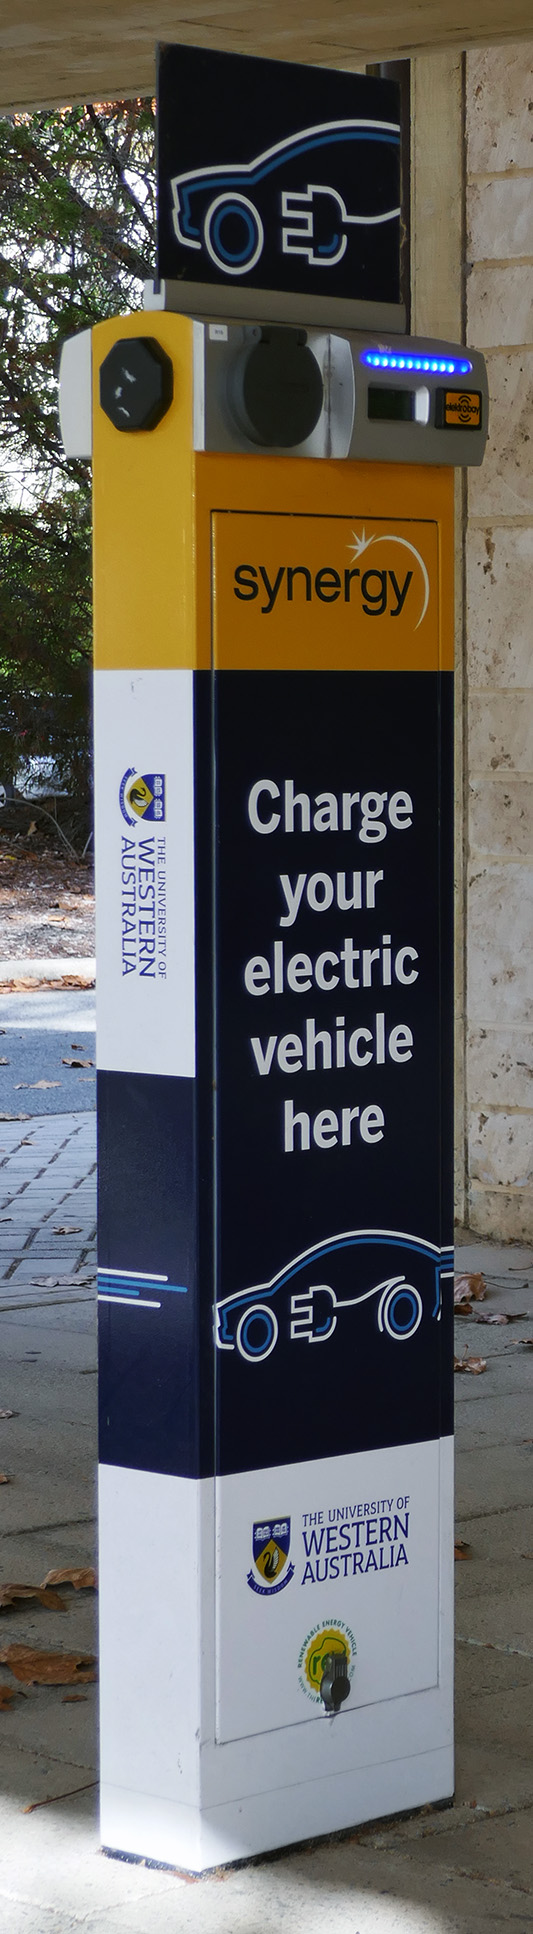
\includegraphics[height=7cm]{accs}
		\caption{AC Charging Station}
		\label{fig:1:accs}   
	\end{subfigure} 
	\hspace{1em}         
	\begin{subfigure}[b]{0.45\textwidth}
		\centering
		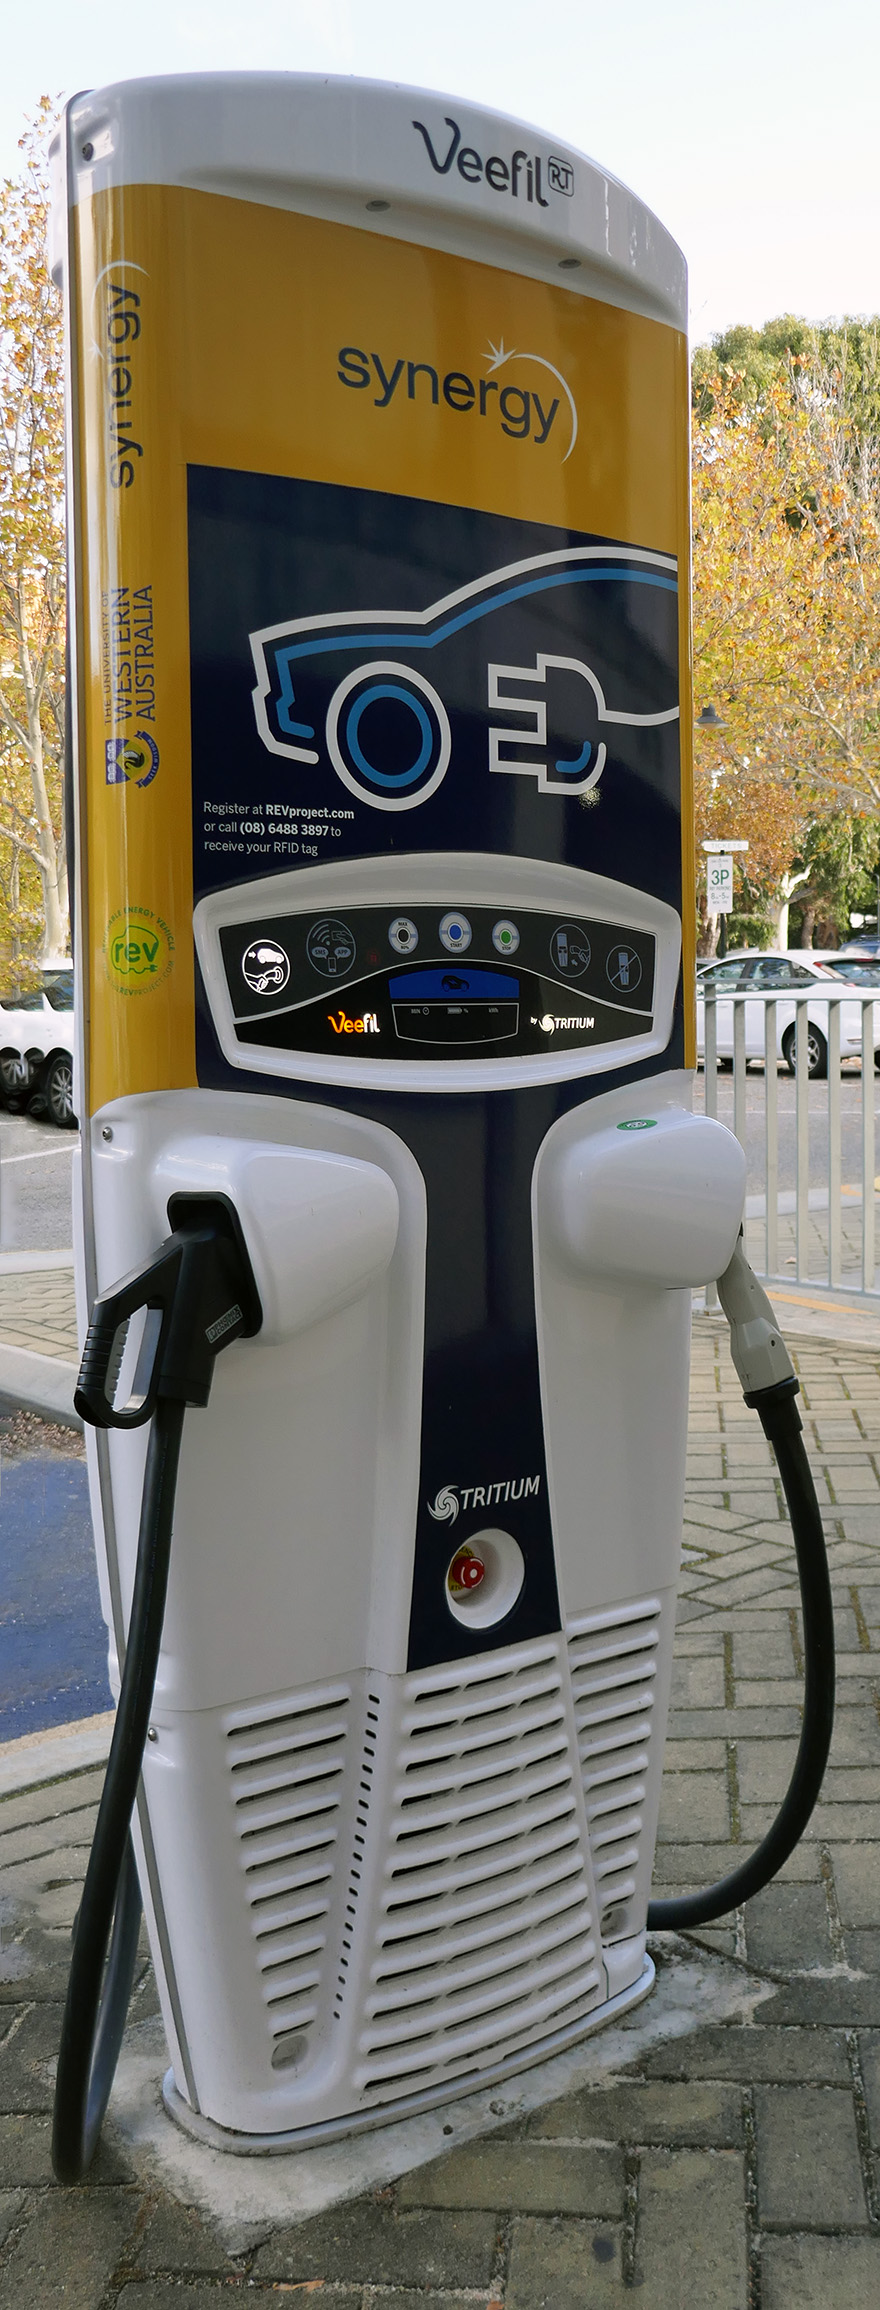
\includegraphics[height=7cm]{dccs}
		\caption{DC Charging Station}
		\label{fig:1:dccs}
	\end{subfigure}             
	\caption{UWA's AC and DC charging stations.}
	\label{fig:1:cs}
\end{figure}

Regulations and incentives have been drafted across various countries either in preparations or in attempts to stimulate EV penetration due to increasing benefits beyond its carbon footprint. These benefits include the running cost of the vehicle, as~\cite{joseph_how_2016} has calculated that an average EV (18 kWh/100 km) is up to five times cheaper to run per kilometre than a typical ICE vehicle (11.1 L/100 km), and are up to 90 per cent more energy efficient. Noting the higher initial cost of EV ownership, many countries have incentivised EV uptakes across varying degrees~\cite{broadbent_electric_2018}. Compared to successful initiatives such as in Norway~\cite{bauer_impact_2018}, the consumer acceptance of EVs is still low in Australia, and researches to encourage local EV uptakes have been limited~\cite{broadbent_analysis_2019}. Notwithstanding, the Australian Senate has established a Select Committee on Electric Vehicles to investigate this issue, resulting in a table of a report~\cite{senate_select_committee_on_electric_vehicles_report_2019}. The notable recommendations presented in this report include a development of national strategy for EVs and charging infrastructures, and setting up a national EV target. Researches in these areas will likely expedite the implementations of the recommendations. 

%https://www.mdpi.com/2032-6653/10/1/11/htm#B2-wevj-10-00011
%https://onlinelibrary.wiley.com/doi/full/10.1111/gec3.12358
%https://www.ergon.com.au/network/smarter-energy/electric-vehicles/charging-your-electric-vehicle

This thesis presents works that address this area through a quantitative analysis of EV charging behaviours using data that was collected from charging stations around Perth. Comparisons are drawn across different charging station types, taking into account a variety of usage scenarios to better visualise the current EV landscape, where it can be used to supplement policy roadmaps to encourage uptake.  
%incentives

\nomenclature[z-unfccc]{UNFCCC}{United Nations Framework Convention on Climate Change} 
\nomenclature[z-ice]{ICE}{Internal combustion engine} 
\nomenclature[z-ev]{EV}{Electric vehicle} 
\nomenclature[z-v2g]{V2G}{Vehicle-to-grid}
\nomenclature[z-iot]{IoT}{Internet of things}

\section{Connected Mobility}
With the availability of low-cost GPS tracking, fleet operators have often relied on vehicle tracking systems to remotely manage and monitor fleets of vehicles. Modern tracking devices are capable of Internet connectivity to transmit telemetry data to a centralised remote server. In addition to location information, this data can include diagnostics from various sensors on the vehicle. In the case of EVs, this can include battery and charging information. 

Further advancements in vehicular communications have incited this to evolve as part of the efforts in vehicle-to-everything (V2X) communications. V2X covers vehicular communication across several aspects including but not limited to V2I (vehicle-to-infrastructure), V2V (vehicle-to-vehicle), V2C (vehicle-to-cloud) and V2G (vehicle-to-grid)~\cite{pearre_review_2019}. These technologies often communicate through a wired or wireless network over a machine to machine (M2M) channel. In the case of wireless connectivity, mobile networks such as 4G are often favoured due to its high transmission speeds, with the incoming 5G standard likely being favoured upon mass deployment, as optimisations are present to facilitate this application. Using mobile networks for V2X applications is often referred to as cellular V2X (C-V2X)~\cite{papathanassiou_cellular_2017}.

With the advent of cloud and edge computing and the Internet of things (IoT), applications pertaining to V2C communications are becoming increasingly prominent, which include the works described in this thesis. V2C has specifically evolved from fleet management systems whereby the addition of a cloud infrastructure presents the application with intelligent control and monitoring~\cite{deng_cooperative_2019}. In the case of an EV ecosystem, a V2C system is capable of consolidating data relating to the EV, charging infrastructures, user behaviours and other stakeholders to present a unified framework for the entire ecosystem. This establishes part of the foundation that leads to intelligent transportation in a smart city, where data from the driving ecosystem is mutually shared for traffic and grid optimisation with low latency connectivity~\cite{hensher_tackling_2018, khattak_toward_2019}, setting the foundation for the Internet of vehicles (IoV).

These communication technologies are easily incorporated into intelligent transportation systems (ITS) to result in smart traffic management and planning; autonomous vehicles will be able to drive cooperatively using a collective perception similar to multi-agent or swarm robotics system. Automotive manufacturers have begun producing vehicles with limited connectivity, but market researches have predicted this market to expand by 45 per cent by 2020 with a 19 per cent CAGR~\cite{market_research_future_connected_2019}. These implications have not gone unnoticed by governments. In Australia, the governments of Western Australia~\cite{weeratunga_connected_2015} and New South Wales~\cite{transport_for_nsw_connected_2018} have studied and produced reports relating to connected vehicles, and the Queensland Government's Cooperative and Automated Vehicle Initiative (CAVI)~\cite{queensland_government_cavi:_2017} has been established to devise policies pertaining to this matter. 

Part of the work described in this thesis intends to establish some preliminary research into connected vehicles in Western Australia. It describes a cloud platform that aggregates data from edge computing that is delivered through a network of smart EV charging stations and an EV fleet. This performs according to a V2C and infrastructure-to-cloud communications system, thereby facilitating data management and reporting to deliver results relating to diagnostics, monitoring and usage forecasts. It is also configured to be extensible to account for the exponential growth in vehicular and infrastructure data, serving as a pragmatic entry into forthcoming big data researches. 

\nomenclature[z-iov]{IoV}{Internet of vehicles} 
\nomenclature[z-m2m]{M2M}{Machine to machine} 
\nomenclature[z-v2x]{V2X}{Vehicle-to-everything} 
\nomenclature[z-v2c]{V2C}{Vehicle-to-cloud} 
\nomenclature[z-v2v]{V2V}{Vehicle-to-vehicle} 
\nomenclature[z-v2x]{V2I}{Vehicle-to-infrastructure} 
\nomenclature[z-v2x]{V2X}{Vehicle-to-everything} 
\nomenclature[z-cavi]{CAVI}{Cooperative and Automated Vehicle Initiative} 
\nomenclature[z-cv2x]{C-V2X}{Cellular vehicle-to-everything} 
\nomenclature[z-4g]{4G}{Fourth generation} 
\nomenclature[z-5g]{5G}{Fifth generation} 

%An example of autonomous driving benefiting from V2V connectivity is through cooperative autonomous driving. This enables a group of vehicles to establish a collective perception, similar to multi agent or swarm robotics systems. 

%The adoption of high-speed wireless connectivity will also benefit autonomous driving, whereby driving decisions and routines including deep learning can be offloaded to a centralised cloud server for processing~\cite{}; traffic management systems can utilise the cloud to achieve adaptive real time performances~\cite{}.

%https://www.sciencedirect.com/science/article/pii/S0967070X17308867
%https://www.mainroads.wa.gov.au/Documents/Connect%20Vehicles%20Web.RCN-D15%5E23413758.PDF
%https://www.future.transport.nsw.gov.au/sites/default/files/media/documents/2019/Connected_and_Automated_Vehicles_Plan.pdf
%https://ieeexplore.ieee.org/abstract/document/8671732
%https://www.marketresearchfuture.com/reports/connected-mobility-solutions-market-871

%With regards to charging speeds, SAE International has published and classified this according to three levels, which Australia follows: 
%
%\begin{itemize}
%	\item Level 1: 2.4 kW AC charging with standard electrical outlets. A full charge is done overnight.
%	\item Level 2: 7.6 kW three-phase AC charging. Three to six hours for a full charge.
%	\item Level 3: Fast DC charging greater than 25 kW. A 350 kW charger typically charges a car in under 10 minutes. 
%\end{itemize}



%li ion fast charging

%paris agreement
%policies
%challenges in area, current state of art, fuel cell
%research question, aims, objective, motivation

%\section{Research Scope}
%This thesis presents its research scope as defined in its aim and objectives. It is multidisciplinary whereby cohesion is given under the context of autonomous electric vehicle applications. 
%
%\subsection{Aim}
%The series of works presented in this thesis aims to formulate pragmatic solutions pertaining to the navigation and charging of electric vehicles by answering the following research questions:
%\begin{enumerate}
%	\item Can autonomous driving be performed using the camera as the primary perceptive sensor?
%	\item How can data from EVs and charging infrastructures be interpreted in a meaningful way?
%\end{enumerate}

\section{Contributions}
The series of works presented in this thesis aims to formulate pragmatic solutions pertaining to the camera as the main sensor for autonomous driving, and interpreting data from EVs and charging infrastructures in a meaningful way. It is multidisciplinary whereby cohesion is ensured under the context of designing system frameworks for autonomous electric vehicle applications. 

To this end, the main contributions of this thesis are summarised as follows:
\begin{itemize}
	\item A literature survey pertaining to visual road recognition with specific emphasises on the methods for autonomous driving applications. Learning methods are presented against conventional methods; recent works relating to academia and the industry are discussed. [Chapter~\ref{ch:vrreview}]
	\item A literature survey pertaining to visual odometry with specific emphasises on autonomous driving applications. These are categorised according to the types of camera used in relation to the current state of research. [Chapter~\ref{ch:voreview}]
	\item An incorporation of visual odometry and semantic segmentation into a multi-robot system. This introduces visual navigation onto an existing system to improve odometric accuracies, and to enable scene understanding for dynamic object recognition. [Chapter~\ref{ch:cmrn}]
	\item An implementation of semantic segmentation on a physical LiDAR-based autonomous driving testbed. This proposed method uses a low-cost monocular camera to segment road regions and lane markings for road centring. [Chapter~\ref{ch:semseg}]
	\item An autonomous driving software framework that is modularly unified to interface sensors with control modules independently. This framework uses protocol buffers to streamline module interoperability to provide an optimised compute performance. [Chapter~\ref{ch:modular}]
	\item A hybrid extension to the aforementioned software framework using Robot Operating System (ROS). Algorithmic additions to path planning and visual navigation are included, along with sensor interfaces and safety functionalities. [Chapter~\ref{ch:evo}]
	\item A hardware-in-the-loop (HIL) simulation system for autonomous driving without real-time constraints. The compute hardware is identical to that used on the autonomous driving testbed using the same ROS integration. [Chapter~\ref{ch:sim}]
	\item A web-based software framework for electromobility telematics. It aggregates and curates data from connected vehicles, charging infrastructures and energy sources, interpreting it for meaningful real-time monitoring and visualisation. [Chapter~\ref{ch:review}]
	\item An analysis of EV charging behaviours on charging stations in Western Australia. Comparisons are drawn across the types and locations of charging stations for their adoption rate, and cost model presented subsequently. [Chapter~\ref{ch:charging}]
\end{itemize}

\nomenclature[z-ros]{ROS}{Robot Operating System} 
\nomenclature[z-hil]{HIL}{Hardware-in-the-loop} 

\section{Thesis Outline}
This thesis comprises of 11 chapters, wherein two chapters present on background reviews, five on autonomous driving frameworks or methods and two on electromobility telematics. The 10 chapters that are subsequent to this introductory chapter are structured as follows: 
%2 survey chapters, 3 on autonomous nav, 2 on electromonbility analysis
\begin{description}
	\item[Chapter~\ref{ch:vrreview}] presents a survey into the current state of research on methods for computer vision-based road recognition. The backgrounds into the methods are first presented categorically according to conventional (non-learning) and machine learning methods, followed by the implementations of these methods. Conventional methods are presented structurally, following common implementations including horizon and vanishing point detection, region of interest isolation, image classification and model fitting; machine learning methods relate to support vector machines and deep learning approaches, covering popular datasets and image segmentation algorithms. These methods are further reviewed for their implementations in relation to autonomous driving. This is presented first as commercial implementations, covering works from corporates and startups, before presenting on recent academic works with practical implementations. 
	\item[Chapter~\ref{ch:voreview}] presents a review on visual odometry methods for autonomous driving across three approaches --- monocular, stereoscopic and visual-inertial. Related applications are discussed for each approach, focusing on works with practical implementations. This is followed by tables that summarise the methods and their presented applications with any applicable datasets. A discussion is drawn to analyse the practicality of the works presented, emphasising on their viability for autonomous driving applications. Through this review it was known that many works truncate upon experimental validations on datasets, and never proceeded with a tangible implementation, leading to a scarcity in their implementations for autonomous vehicles. This chapter concludes by drawing the necessity of such implementations, as the dynamism of real-world environments must be accounted for.
	\item[Chapter~\ref{ch:cmrn}] describes an implementation of visual odometry and semantic segmentation onto a multi-robot system. The proposal of this implementation acts as a preliminary testbed for the visual navigation algorithms to test their application feasibility before they are ported onto an actual road vehicle. In addition, the incorporation of these algorithms intends to improve upon the existing multi-robot system's localisation accuracy, as well as supplementing navigation with scene understanding. In particular, as the existing system localises upon wheel odometry, the introduction of visual odometry intends to mitigate the error accumulation caused by wheel slip, a common problem that occurs in wheel odometry systems. Navigation on the system is performed in a decentralised manner, such that navigational algorithms run independently on each robot without relying on an external or central computer. Evaluations on the visual navigation algorithms have ascertained the feasibility of their implementations in solving problems relating to odometry and object classification while being resilient against environmental dynamics. 
	\item [Chapter~\ref{ch:semseg}] focuses on the application of a semantic segmentation method onto an autonomous driving testbed. The existing testbed is equipped with a LiDAR for object detection, and the addition of visual navigation intends to supersede that to achieve scene understanding and object perceptibility. A low-cost USB camera is mounted onto the vehicle's frame, where it and the other sensors are physically calibrated for camera-LiDAR distance measurements. Semantic segmentation is then applied to the camera recordings and its pixel accuracy is subsequently measured. Experimental results have shown that segmentation is adequate for road markings and lane detection on Perth roads. 
	\item [Chapter~\ref{ch:modular}] explores the first iteration for an improved software framework for the autonomous driving testbed. The original framework heavily relied on a central Control module which required all sensors and submodules to run. The proposed framework is more efficient whereby it is programmed using a C++ interface across all modules. Existing modules are either translated or reprogrammed, which streamlines and optimises individual algorithms to run on the testbed's embedded computer, enabling high performances throughout the software architecture. Module interoperability is ensured using protocol buffers, which separate them into independent classes. Experimental results have validated the efficiency of the software framework, which is given in outputs relating to localisation, odometry, path planning, control and semantic segmentation. 
	\item [Chapter~\ref{ch:evo}] proposes a hybrid enhancement to the C++-based software framework as a high-level control system. This new framework is based on ROS, and modularly combines sensor data and navigation processing for autonomous driving, while simultaneously ensures vehicle safety and provides data visualisation. %The navigation sensors achieve of wheel odometry, dead reckoning, LiDAR and camera detection
	It is capable of navigating along with a set of predefined waypoints, or along a cone-delimited path. Visual navigation is once again presented for road and lane detection using semantic segmentation, visual odometry and cone tracking. A HIL simulator is also presented to introduce a parallel development platform using identical compute hardware. Experiments were conducted for sensor fusion, waypoint driving, cone driving and the simulator, where results have collectively demonstrated the system's robustness and adequacy for practical implementations. 
	\item [Chapter~\ref{ch:sim}] expands on the HIL simulation system described to elaborate on its features. Using a HIL system enables algorithmic prototyping to be rapidly deployed while reducing such risks when compared to a physical system. This is a CARLA-based simulation system at the front-end, whereas autonomous driving routines are performed using identical ROS-based compute hardware across real-world and simulation testbeds to illustrate realistic constraints in relation to its computation footprint. This include using identical ROS modules for LiDAR point clouds and camera visualisations. Comparisons were made between the simulation and the physical system, with articulations on the cone detection (LiDAR and vision-based) and path planning algorithms. Evaluations were drawn to benchmark these algorithms, in addition to vehicle dynamics and computation requirements, where it was verified that the tests conducted are transferable between physical and simulation systems.
	\item [Chapter~\ref{ch:review}] introduces the electromobility research in this thesis by detailing the software framework used to collect and process telemetry data from various EVs and their infrastructures. A centralised cloud server is developed for this telematics platform which EVs, charging infrastructures and power sources push data to. The application layer is entirely web-based and is capable of pulling data in real-time for user monitoring and visualisations. This is presented for charging stations, EV fleet tracking and energy generation, wherein for each section, the back-ends and algorithms are elaborated to result in visualisations. Gamification is presented for vehicle tracking to encourage economical driving, and monetisation options are presented as bills to inform users of energy usage in charging stations. The results generated from this telematics platform were summarised as usages pertaining to charging infrastructures and energy generation, as well as heat maps for EV tracking. A forecast of the charging infrastructures' usage is also presented and analysed as a precursor to predicting the local EV penetration. All platform modules were written in a modular approach to encourage future improvements and expansions.  
	\item [Chapter~\ref{ch:charging}] investigates EV charging behaviours by analysing data on the telemetry platform. This begins with a background on various types of EV charging worldwide, followed by charging speeds and cycles. Data is collected from charging stations managed by The REV Project, with comparisons drawn using data from the RAC Electric Highway in Western Australia. Data is analysed through various time series analysis, which investigated station usage frequencies and energy consumption over a predefined period; samples are given in hours-of-day and days-of-week to study usage patterns. A cost model is drawn to estimate the costs for running and maintaining different types of charging stations, and external scenarios such as parking bay rentals are also considered. These analyses are validated using a similar study, and it was concluded that slower charging stations are becoming obsolete and are shifting towards personal installations, whereas public installations will prefer fast-charging stations. 
	\item [Chapter~\ref{ch:conclu}] concludes this thesis with a summary of the contributions made, along with suggestions to outline future research directions.
\end{description}

%focuses, targets, 

%%!TEX root = ../thesis.tex
%%*******************************************************************************
%%*********************************** First Chapter *****************************
%%*******************************************************************************
%
%\chapter{Getting started}  %Title of the First Chapter
%
%\ifpdf
%    \graphicspath{{Chapter1/Figs/Raster/}{Chapter1/Figs/PDF/}{Chapter1/Figs/}}
%\else
%    \graphicspath{{Chapter1/Figs/Vector/}{Chapter1/Figs/}}
%\fi
%
%
%%********************************** %First Section  **************************************
%\section{What is loren ipsum? Title with math \texorpdfstring{$\sigma$}{[sigma]}} %Section - 1.1 
%
%Lorem Ipsum is simply dummy text of the printing and typesetting industry (see 
%Section~\ref{section1.3}). Lorem Ipsum~\citep{Aup91} has been the industry's 
%standard dummy text ever since the 1500s, when an unknown printer took a galley 
%of type and scrambled it to make a type specimen book. It has survived not only 
%five centuries, but also the leap into electronic typesetting, remaining 
%essentially unchanged. It was popularised in the 1960s with the release of 
%Letraset sheets containing Lorem Ipsum passages, and more recently with desktop 
%publishing software like Aldus PageMaker including versions of Lorem 
%Ipsum~\citep{AAB95,Con90,LM65}.
%
%The most famous equation in the world: $E^2 = (m_0c^2)^2 + (pc)^2$, which is 
%known as the \textbf{energy-mass-momentum} relation as an in-line equation.
%
%A {\em \LaTeX{} class file}\index{\LaTeX{} class file@LaTeX class file} is a file, which holds style information for a particular \LaTeX{}.
%
%
%\begin{align}
%CIF: \hspace*{5mm}F_0^j(a) = \frac{1}{2\pi \iota} \oint_{\gamma} \frac{F_0^j(z)}{z - a} dz
%\end{align}
%
%\nomenclature[z-cif]{$CIF$}{Cauchy's Integral Formula}                                % first letter Z is for Acronyms 
%\nomenclature[a-F]{$F$}{complex function}                                                   % first letter A is for Roman symbols
%\nomenclature[g-p]{$\pi$}{ $\simeq 3.14\ldots$}                                             % first letter G is for Greek Symbols
%\nomenclature[g-i]{$\iota$}{unit imaginary number $\sqrt{-1}$}                      % first letter G is for Greek Symbols
%\nomenclature[g-g]{$\gamma$}{a simply closed curve on a complex plane}  % first letter G is for Greek Symbols
%\nomenclature[x-i]{$\oint_\gamma$}{integration around a curve $\gamma$} % first letter X is for Other Symbols
%\nomenclature[r-j]{$j$}{superscript index}                                                       % first letter R is for superscripts
%\nomenclature[s-0]{$0$}{subscript index}                                                        % first letter S is for subscripts
%
%
%%********************************** %Second Section  *************************************
%\section{Why do we use loren ipsum?} %Section - 1.2
%
%
%It is a long established fact that a reader will be distracted by the readable content of a page when looking at its layout. The point of using Lorem Ipsum is that it has a more-or-less normal distribution of letters, as opposed to using `Content here, content here', making it look like readable English. Many desktop publishing packages and web page editors now use Lorem Ipsum as their default model text, and a search for `lorem ipsum' will uncover many web sites still in their infancy. Various versions have evolved over the years, sometimes by accident, sometimes on purpose (injected humour and the like).
%
%%********************************** % Third Section  *************************************
%\section{Where does it come from?}  %Section - 1.3 
%\label{section1.3}
%
%Contrary to popular belief, Lorem Ipsum is not simply random text. It has roots in a piece of classical Latin literature from 45 BC, making it over 2000 years old. Richard McClintock, a Latin professor at Hampden-Sydney College in Virginia, looked up one of the more obscure Latin words, consectetur, from a Lorem Ipsum passage, and going through the cites of the word in classical literature, discovered the undoubtable source. Lorem Ipsum comes from sections 1.10.32 and 1.10.33 of "de Finibus Bonorum et Malorum" (The Extremes of Good and Evil) by Cicero, written in 45 BC. This book is a treatise on the theory of ethics, very popular during the Renaissance. The first line of Lorem Ipsum, "Lorem ipsum dolor sit amet..", comes from a line in section 1.10.32.
%
%The standard chunk of Lorem Ipsum used since the 1500s is reproduced below for those interested. Sections 1.10.32 and 1.10.33 from ``de Finibus Bonorum et Malorum" by Cicero are also reproduced in their exact original form, accompanied by English versions from the 1914 translation by H. Rackham
%
%``Lorem ipsum dolor sit amet, consectetur adipisicing elit, sed do eiusmod tempor incididunt ut labore et dolore magna aliqua. Ut enim ad minim veniam, quis nostrud exercitation ullamco laboris nisi ut aliquip ex ea commodo consequat. Duis aute irure dolor in reprehenderit in voluptate velit esse cillum dolore eu fugiat nulla pariatur. Excepteur sint occaecat cupidatat non proident, sunt in culpa qui officia deserunt mollit anim id est laborum."
%
%Section 1.10.32 of ``de Finibus Bonorum et Malorum", written by Cicero in 45 BC: ``Sed ut perspiciatis unde omnis iste natus error sit voluptatem accusantium doloremque laudantium, totam rem aperiam, eaque ipsa quae ab illo inventore veritatis et quasi architecto beatae vitae dicta sunt explicabo. Nemo enim ipsam voluptatem quia voluptas sit aspernatur aut odit aut fugit, sed quia consequuntur magni dolores eos qui ratione voluptatem sequi nesciunt. Neque porro quisquam est, qui dolorem ipsum quia dolor sit amet, consectetur, adipisci velit, sed quia non numquam eius modi tempora incidunt ut labore et dolore magnam aliquam quaerat voluptatem. Ut enim ad minima veniam, quis nostrum exercitationem ullam corporis suscipit laboriosam, nisi ut aliquid ex ea commodi consequatur? Quis autem vel eum iure reprehenderit qui in ea voluptate velit esse quam nihil molestiae consequatur, vel illum qui dolorem eum fugiat quo voluptas nulla pariatur?"
%
%1914 translation by H. Rackham: ``But I must explain to you how all this mistaken idea of denouncing pleasure and praising pain was born and I will give you a complete account of the system, and expound the actual teachings of the great explorer of the truth, the master-builder of human happiness. No one rejects, dislikes, or avoids pleasure itself, because it is pleasure, but because those who do not know how to pursue pleasure rationally encounter consequences that are extremely painful. Nor again is there anyone who loves or pursues or desires to obtain pain of itself, because it is pain, but because occasionally circumstances occur in which toil and pain can procure him some great pleasure. To take a trivial example, which of us ever undertakes laborious physical exercise, except to obtain some advantage from it? But who has any right to find fault with a man who chooses to enjoy a pleasure that has no annoying consequences, or one who avoids a pain that produces no resultant pleasure?"
%
%Section 1.10.33 of ``de Finibus Bonorum et Malorum", written by Cicero in 45 BC: ``At vero eos et accusamus et iusto odio dignissimos ducimus qui blanditiis praesentium voluptatum deleniti atque corrupti quos dolores et quas molestias excepturi sint occaecati cupiditate non provident, similique sunt in culpa qui officia deserunt mollitia animi, id est laborum et dolorum fuga. Et harum quidem rerum facilis est et expedita distinctio. Nam libero tempore, cum soluta nobis est eligendi optio cumque nihil impedit quo minus id quod maxime placeat facere possimus, omnis voluptas assumenda est, omnis dolor repellendus. Temporibus autem quibusdam et aut officiis debitis aut rerum necessitatibus saepe eveniet ut et voluptates repudiandae sint et molestiae non recusandae. Itaque earum rerum hic tenetur a sapiente delectus, ut aut reiciendis voluptatibus maiores alias consequatur aut perferendis doloribus asperiores repellat."
%
%1914 translation by H. Rackham: ``On the other hand, we denounce with righteous indignation and dislike men who are so beguiled and demoralized by the charms of pleasure of the moment, so blinded by desire, that they cannot foresee the pain and trouble that are bound to ensue; and equal blame belongs to those who fail in their duty through weakness of will, which is the same as saying through shrinking from toil and pain. These cases are perfectly simple and easy to distinguish. In a free hour, when our power of choice is untrammelled and when nothing prevents our being able to do what we like best, every pleasure is to be welcomed and every pain avoided. But in certain circumstances and owing to the claims of duty or the obligations of business it will frequently occur that pleasures have to be repudiated and annoyances accepted. The wise man therefore always holds in these matters to this principle of selection: he rejects pleasures to secure other greater pleasures, or else he endures pains to avoid worse pains."
%
%\nomenclature[z-DEM]{DEM}{Discrete Element Method}
%\nomenclature[z-FEM]{FEM}{Finite Element Method}
%\nomenclature[z-PFEM]{PFEM}{Particle Finite Element Method}
%\nomenclature[z-FVM]{FVM}{Finite Volume Method}
%\nomenclature[z-BEM]{BEM}{Boundary Element Method}
%\nomenclature[z-MPM]{MPM}{Material Point Method}
%\nomenclature[z-LBM]{LBM}{Lattice Boltzmann Method}
%\nomenclature[z-MRT]{MRT}{Multi-Relaxation 
%Time}
%\nomenclature[z-RVE]{RVE}{Representative Elemental Volume}
%\nomenclature[z-GPU]{GPU}{Graphics Processing Unit}
%\nomenclature[z-SH]{SH}{Savage Hutter}
%\nomenclature[z-CFD]{CFD}{Computational Fluid Dynamics}
%\nomenclature[z-LES]{LES}{Large Eddy Simulation}
%\nomenclature[z-FLOP]{FLOP}{Floating Point Operations}
%\nomenclature[z-ALU]{ALU}{Arithmetic Logic Unit}
%\nomenclature[z-FPU]{FPU}{Floating Point Unit}
%\nomenclature[z-SM]{SM}{Streaming Multiprocessors}
%\nomenclature[z-PCI]{PCI}{Peripheral Component Interconnect}
%\nomenclature[z-CK]{CK}{Carman - Kozeny}
%\nomenclature[z-CD]{CD}{Contact Dynamics}
%\nomenclature[z-DNS]{DNS}{Direct Numerical Simulation}
%\nomenclature[z-EFG]{EFG}{Element-Free Galerkin}
%\nomenclature[z-PIC]{PIC}{Particle-in-cell}
%\nomenclature[z-USF]{USF}{Update Stress First}
%\nomenclature[z-USL]{USL}{Update Stress Last}
%\nomenclature[s-crit]{crit}{Critical state}
%\nomenclature[z-DKT]{DKT}{Draft Kiss Tumble}
%\nomenclature[z-PPC]{PPC}{Particles per cell}